\newchapt{Keyslice Detection}{chapt4}{Keyslice Detection}

%%%%%%%%%%%%%%%%%%%%%%%%%%%%%%%%
%%%%%%   3D Reconstruction  %%%%
%%%%%%%%%%%%%%%%%%%%%%%%%%%%%%%%
%\section{Lightweight 3D Reconstruction}
\label{sec:reconst}
Our 3D modeling algorithm is based on \emph{a priori} knowledge that
urban buildings can be created through a series of extrusion and taper
operations on the salient cross-sections contained in the keyslices.
\Fig{keyslices} depicts the keyslices derived from the uniform slices
given in \Fig{slice_slab}. 
The key step for successful modeling is identifying these salient cross
sections upon which the extrusion and taper operations will apply.

An intuitive way for key slice detection is to compute the similarity between the sliced images.
In other words, the sliced images are clustered into different groups based on the similarity among them.
There are two mainly research methods for similarity measurement of 2D images: area based method and feature based
methods. The area based methods are computational efficient but they usually can only be applied on
binary or gray-scale images. The feature based one is computational complex but more powerful and can be applied
to images obtained using different sensors, such as multi-modal image registration.
% read similarity measure papers.
Because our goal is to develop light-weight efficient algorithm for model reconstruction, plus
the input for similarity measure is pure binary images, the area based method is adopted for our approach.

The classical measure for area based method is the normalized cross
correlation \cite{DIP_Pratt}:
\begin{equation*}
CC(i,j) = \frac{\sum_W(W - E(W))(I_{(i,j)}-E(I_{(i,j)}))}
{\sqrt{\sum_W(W - E(W))^2}\sqrt{\sum_{I_{(i,j)}}(I_{(i,j)} - E(I_{(i,j)}))^2}}
\end{equation*}
where $W$ is an image mask, $E(W)$ is the mean of the mask's pixels, and $E(I_{(i,j)})$
is the mean of the image pixels covered by the mask $W$.
However, this method is very time consuming and is a local window-based approach,
which could not capture the global relations between images. Therefore, we proposed a
light-weighted global and efficient key image detection approach based on Hausdorff distance 
and curvatures computation.

\begin{figure}[hbtp]
\centering
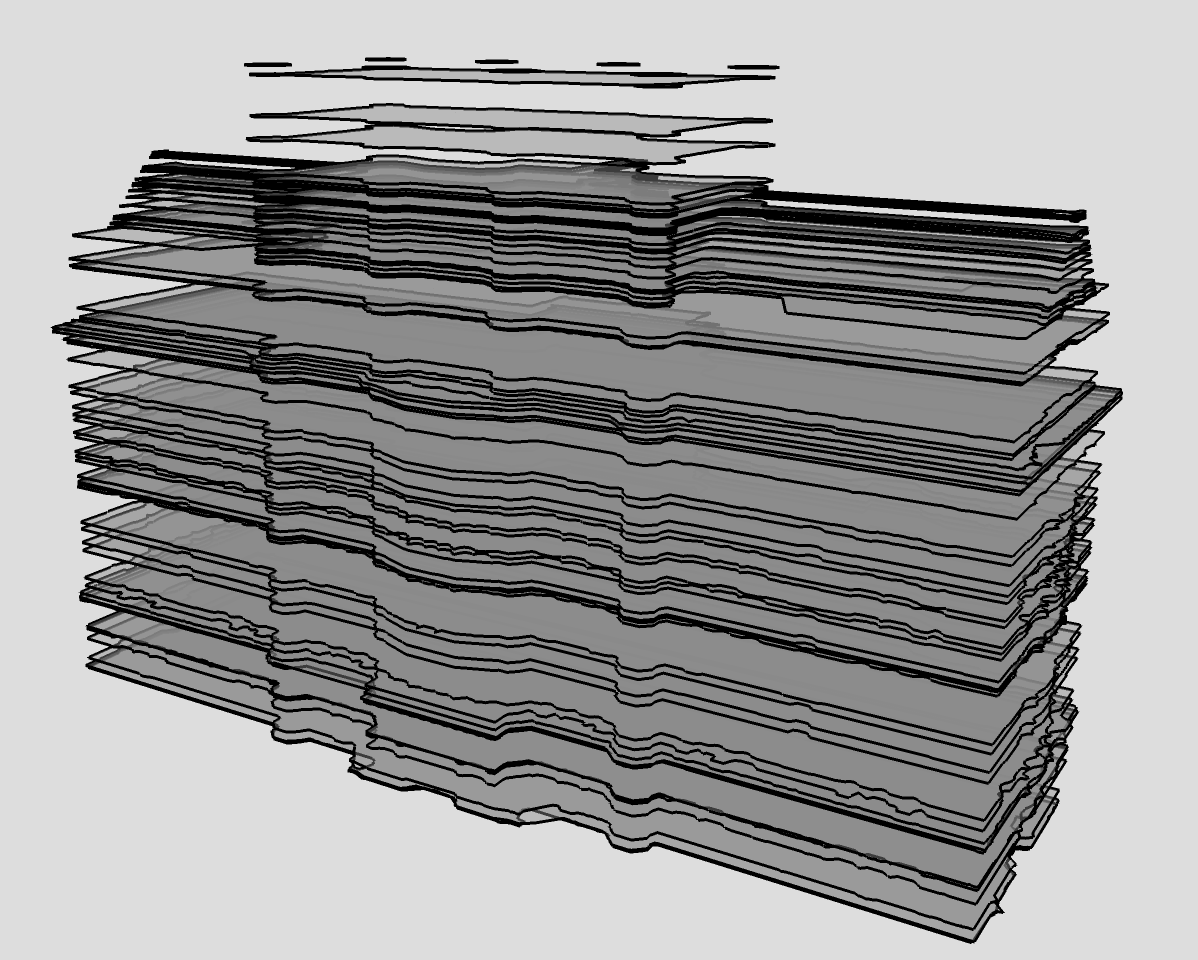
\includegraphics[width=0.8\textwidth]{figures/keyslice_wireframe.png}
\caption{Keyslices derived from the input in \Fig{slice_slab}.}
\label{fig:keyslices}
\end{figure}

\section{Hausdorff Distance Based}
\label{sec:ksd}
The 2D image slices of an extruded region are similar to each other.
Thus, to detect the keyslices that delimit extruded regions one only needs
to compute the similarity between adjacent slices.
We select the Hausdorff distance \cite{IR_HKR} as the similarity measure.
Let $P_r(x_r, y_r)$ be a data point in a reference image and
let $P_i(x_i, y_i)$ be a data point in a new observed image $I$.
The Hausdorff distance of image $I$ to reference image $I_r$ is defined as:

\begin{equation}
d_H(I, I_r) = \sum_{i=0}^Nd_{min}(P_i, I_r)
\label{eq:hd}
\end{equation}

where $d_{min}(P_i, I_r)$ is the minimum distance from data point $P_i$
in image $I$ to the reference image $I_r$.
Alternatively, we can also define the Hausdorff distance, $d_H(I_r, I)$,
from reference image $I_r$ to a new observed image $I$, using \Eq{hd}.
These two distances are usually not equal to each other.
As a rule of thumb, one can choose
$d_{HD} = \text{MAX}\{d_H(I, I_r), d_H(I_r, I)\}$ as the Hausdorff distance.
To compute the keyslices, a threshold $\tau_{d}$ is used for the
Hausdorff distance $d_{HD}$.
If $d_{HD} < \tau_{d}$, the two images $I$ and $I_r$ are considered
similar to each other.
Otherwise, a keyslice image is found and $I_r$ is updated with $I$,
the new keyslice image.

\section{Curvature Based}
The accuracy of the keyslices detected by using the Hausdorff distance
is closely tied to threshold $\tau_d$.
Small $\tau_d$ leads to more accurate models and will require more time and
space to compute and store the result.
When the threshold $\tau_d$ is relatively large, potential keyslices which
contain salient structure may be missed.
Therefore, there is a trade-off between model accuracy and time-space
efficiency.
To address this problem, the curvature information is computed as a
complementary criteria for keyslice detection.

This idea is based on the observation that the keyslices are generally
located at large curvature changes along 2D slices extracted in the orthogonal
direction (e.g., side view), as shown in \Figa{HT_BPA_Curvature}.
Therefore, instead of computing the difference between two images directly,
we compute the curvature of orthogonal 2D slices, map the positions of
curvature extrema back to cross-sections in the original set of volumetric
slabs, and mark these cross-sections as keyslices.

\begin{figure}[htbp]
\begin{center}
\begin{tabular}{cc}
\fbox{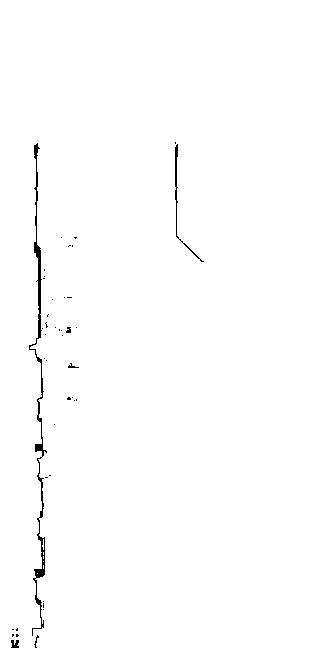
\includegraphics[width=0.3\textwidth]{image_slice_lr_0580_0590_half.jpg}}
\fbox{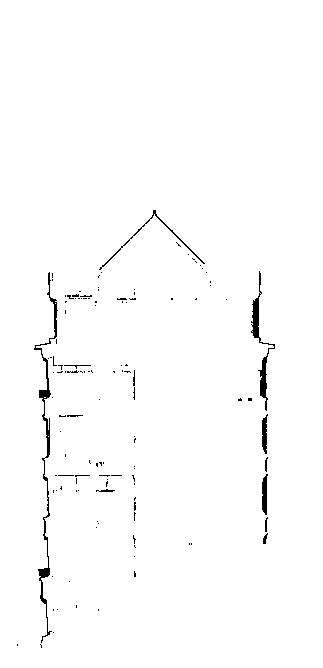
\includegraphics[width=0.3\textwidth]{image_slice_lr_0830_0842_half.jpg}} &
\fbox{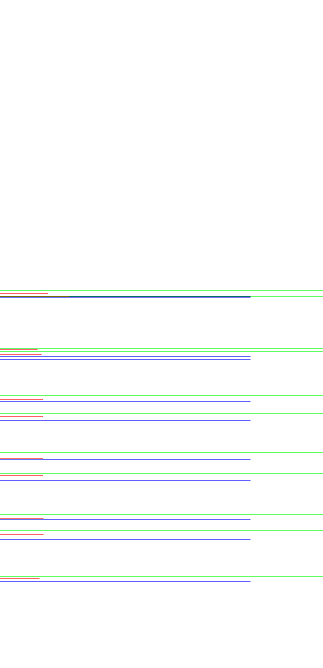
\includegraphics[width=0.3\textwidth]{curvature_center_lines_old_half.jpg}} \\
(a) & (b)
\end{tabular}
\end{center}
\caption{Curvature-based key slice detection.
(a) A partial set of two 2D sliced images from the orthogonal direction (side
view). The complete set will be used to extract the keyslices shown in
\Fig{keyslices}.
(b) The average curvatures detected over all of the sliced images along the
orthogonal direction.}
\label{fig:HT_BPA_Curvature}
\end{figure}

In the close-up view of a small region as shown in \Fig{KSD_Curv},
two curvatures, $c_1$ and $c_2$, are
computed in this small region. The red, blue and green lines indicate the locations
of the center, the starting and the ending of a curvature. 
As a matter of fact, there is a third curvature computed around the
black box sitting on top of the green line of the curvature $c_1$. 
However, this third one should not be consider as a real curvature 
in that the black box is due to an air conditioner during the data acquisition process, 
which means it is not a part of the building. We called this third curvature
{\it outlier curvature} which needs to be removed from the set of real curvatures.
Based on the fact that these outlier curvatures exist only in a few 2D slices,
we can exclude them by counting the number of appearance for each curvature.
Only those curvatures appears in most of the 2D slices are kept for further computation.

Once the real curvatures are obtained, they can be used as a complemental way of 
Hausdorff distance for keyslices detection. 
Each curvature $c$ is mapped to a set $s$ of original 2D cross-sectional
slices, $i,\ldots,j$, where $i$ and $j$ are corresponding to the starting and 
the ending locations of $c$. After this, the set $s$ is checked whether 
it contains any keyslice or not.
If a keyslice $k$ has been marked in $s$ by Hausdorff distance, 
nothing needs to be done and this curvature $c$ is discarded. 
On the other hand, if $s$ contains no keyslice, $i$ and $j$ will be marked as 
two new keyslices to keep the salient feature identified by this curvature $c$.
The combination of Hausdorff distance measurement and curvature inference
ensures that the salient structures of a building will be preserved.

%%% Figure of the tapered template.
\begin{figure}[htbp]
\begin{center}
\begin{tabular}{c}
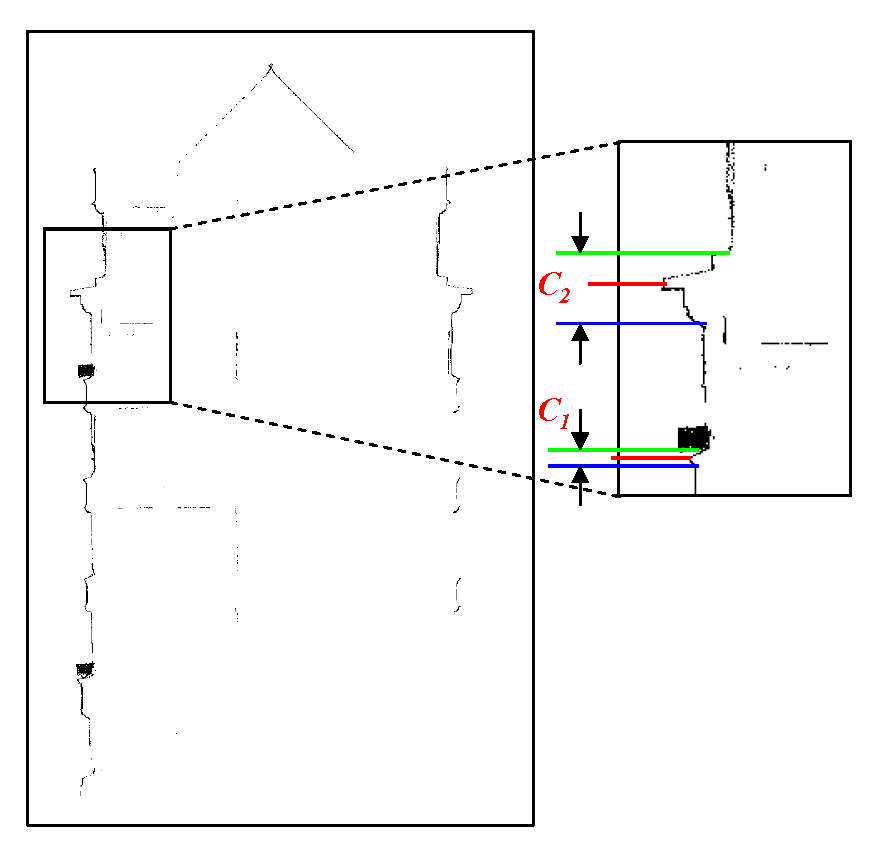
\includegraphics[width=0.60\textwidth]{curvature.png}
\end{tabular}
\end{center}
\caption{ Curvature based key slice detection. }
\label{fig:KSD_Curv}
\end{figure}
%%% End of Figure

To compute the curvature, we first apply the slice extraction algorithm
described in \Sec{image_slicing} to obtain a series of 2D cross-sectional
images in the orthogonal direction.
We then apply the ball-pivot algorithm described in \Sec{BPA} to
vectorize the boundary for each sliced image.
We locate those curvatures that appear in most of the sliced images as the
places where keyslices are found, as shown in \Figb{HT_BPA_Curvature}.
Note that the red lines indicate location of the center of the curvature,
and the blue and green lines indicate the entering and exiting of the
curvature structures, respectively.
The combination of Hausdorff distance measurement and curvature inference
ensures that the salient structures of a building will be preserved.

\section{Loal Matching Based on Segmentation}

The keyslice detection described above are based on global information matching.
The strength of these methods lies on the effective of computation and they can
also produce good results on exterior scanning as depicted in \Fig{keyslices}. 
However, when applied to interior scannings when the layout of the structures 
is complex, there may be some limitations on these methods. 
As depicted in \Fig{ksd_gbl_bad}, the pillars inside the hall can be reconstructed
by simple extrusion of the base polygon. However, they are divided to 
excessive amount of keyslices because the dissimilarity of the outside window
structures in the same projection level. In other words, due to global matching
strategy, some independent objects which could be modeled using simple extrusion
operation are modeling using excessive keyslices. Although the reconstructed
models are still correct at this situation, they are not efficiency. That is, much
more keyslices are created to represent the simpled extruded parts. 

A more effective way for modeling the above structures is to model the different 
structures individually. By doing this, we can simply model the pillars using a
extrusion operation based on a base polygon. Certainly, for the complicate window
structures, more keyslices are still required but these keyslices would not contain
any pillar structures. To do this, segmentation is a necessary step to identify
all different parts of the scannings. 

There are a lot of literatures on image segmentation as in \cite{segmentation}. 
% a little bit survey on image segmentation, especially binary image segmentation.
% why the graph-cut is well-fit for our purpose.

Our segmentation based keyslice detection approach is an iterative algorithm.
We first applied the graph cut
on the 2D sliced binary image. The initial input to graph cut is done as follows. 
First of all, a random data point $p$ was located in the binary image $I$. The data
point $p$ is then growing to form an region $r$ based on the connected components 
until it reaches a fix-point. That is, no more data point can be reached in $r$. $r$
is taken as input by graph cut algorithm to compute the segmentations. 
The segmented objects (non-background pixels) are then stored and their pixels are 
reset to background pixels for next iteration. The algorithm is depicted in \Fig{alg_seg}.
To adjust the accuracy of the graph cut, the parameter ??? was used. To get more
accurate segments, which means more objects may be classified, enlarge/shrink its value.

For each new 2D image slice, there is a set of segmented objects $s$ is computed
by the above graph cut approach. Therefore, the keyslice detection problem is converted
into similarity measurement of the detected segments along the specified direction, 
e.g., vertical direction.
The similarity measurement is now among the segmented regions instead of the whole
contour of a sliced image. A global data structure, $T$, which contains all the current 
active segmented objects is maintained for matching. $T$ is initialized with the
detected segments from the first 2D slice which is regared as reference slice. 

For each new observed 2D slice, we first compute a set of segmented objects $s$. 
After this, we are trying to search for a matched segmented object $o'$ in $s$ for 
each existed active segmented objects $o$ in $T$. This searching process again is 
based on the Hausdorff distance described in \ref{ksd}. If such a matched object $o'$
exists, $o$ will be kept in $T$ as an active segmented object for next round of
computation. Otherwise, $o$ is removed from $T$ and is treated as a completed part or
object in the range data. At the same time, for any object $o'$ in $s$, if it is 
not found to be a matched segments for active objects in $T$, $o'$ will be added
to $T$ as a starting slice of a new part in range data and will be taken into
account for next adjance 2D slice computation. We keep doing this until the last
2D slice is visited and processed. Once the last slice is reached, all the active
segments in $T$ will be considered as the ending point of the objects in the range data.

The result obtained by the aboved local based keyslice detection is illustrated in 
\Fig{ksd_lcl_good}. As we can see, the pillar structures of the hall are reconstructed
using the simple extrusion operations, which is much more efficienct in terms of 
model size and representation.







